%!TEX root = ../disertace.tex
%!TEX encoding = UTF-8 Unicode

\chapter{\seman}
\label{sec:seman}
The annotation tool \seman\ is written in Perl 5\footnote{\url{www.perl.org}; \url{dev.perl.org/perl5}} with Perl/Tk\footnote{\url{http://search.cpan.org/~srezic/Tk-804.029/}} GUI toolkit. The annotation tool depends on working installation of \tred, specifically its unix installation, because it uses \texttt{nTrEd} for efficient execution of \tred\ scripts in the background. \texttt{nTrEd} however, unlike \tred\ itself or \texttt{bTrEd}, does not work on Windows.% because it uses unix sockets.

 \seman\ itself is composed of several main parts:
\begin{itemize}
  \item The main application file \code{sem-ann.pl} mostly implements the application frontend. It implements the GUI, loads an \sf, a \semlex,  and a log file for this \sf, if it had already been annotated. Then it takes care of all the interaction with the user and writes \sf, \semlex, and a log file.
  \item \ntred\ backend that is used to 
	\begin{itemize}
	  \item generate surface sentences from tectogrammatical trees in \tf{}s that are then displayed in the \seman\ GUI,
	  \item perform all the on-the fly pre-annotations (\Sref{sec:annot:pre})
	\end{itemize}
	What we call ``backend'' is thus the running \ntred\ instance itself (that is run by the \seman\ during start-up), and the scripts used to generate the sentences that are displayed in \seman\ and to pre-annotate MWEs using their tectogrammatical tree structures.\footnote{these scripts were written entirely by E. Bejček~(\citeyear{bejcek:2010}).}
  \item The module \code{SemLex.pm} is used to read, save, query, and edit \semlex.
    \item The module \code{SemLex\textunderscore{}heslo.pm} implements the \semlex\ entry: its structure, attributes and accessors.
  \item There is also a suite of miscellaneous scripts mostly for validation of annotated data, comparing and merging multiple annotations, merging annotators' \semlex{}es, computing reliability of annotations, and other small tasks related to annotation and managing the annotated data and \semlex{}es.
\end{itemize}

\section{User interface}
\label{sec:seman:gui}
The user interface (shown in \Fref{fig:seman-gui}) is divided into three main parts (top to bottom):

\subsection{Key bindings}


\section{Annotation logs}
\label{sec:logs}


% sem-ann screenshot 
\begin{figure}[htbp]
   \centering
   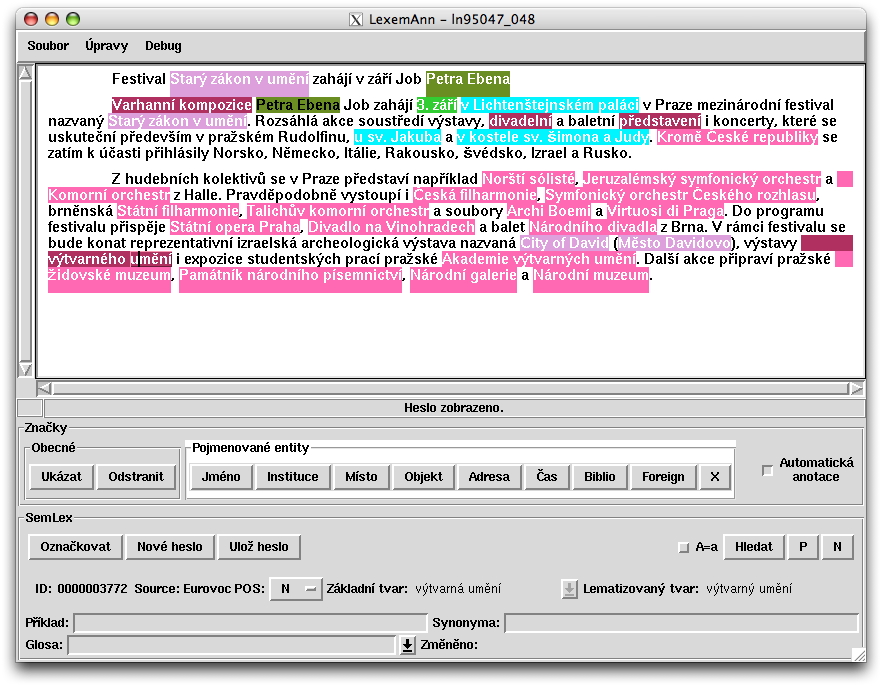
\includegraphics[scale=.4]{images/sem-ann.png} 
   \caption{An annotated document in \seman. the ``\code{sel}''-- selection tag is barely visible on the word \pr{umění} (second word from the left, second line from the bottom). The \semlex\ entry that is displayed in the Semlex-part of the UI -- \pr{výtvarná umění} -- is the one used to annotate the selected word. }
   \label{fig:seman-gui}
\end{figure}